% Prepared by Calvin Kent
%
% Assignment Template v19.02
%
%%% 20xx0x/MATHxxx/Crowdmark/Ax
%
\documentclass[12pt]{article} %
\usepackage{CKpreamble}
\usepackage{CKassignment}
\usepackage{tkz-euclide}
\usepackage{physunits}
\usepackage{physics}
\usepackage{lmodern}
\usepackage{microtype}
\usepackage{upgreek}
\usepackage[misc]{ifsym}
\title{Physics 11 Test 1 - \textbf{SOLUTION} \\ \textbf{Time : 1.5 hrs}}
\date{2021\\ August}
\author{Abdullah Zubair}

%%% Maths and science packages

\usepackage{amsmath,amsthm,amssymb}
\usepackage{pgfplots}
	\usetikzlibrary{
		calc,
		patterns,
		positioning
	}
	\pgfplotsset{
		compat=1.16,
		samples=200,
		clip=false,
		my axis style/.style={
			axis x line=middle,
			axis y line=middle,
			legend pos=outer north east,
			axis line style={
				->,
			},
			legend style={
				font=\footnotesize
			},
			label style={
				font=\footnotesize
			},
			tick label style={
				font=\footnotesize
			},
			xlabel style={
				at={
					(ticklabel* cs:1)
				},
				anchor=west,
				font=\footnotesize,
			},
			ylabel style={
				at={
					(ticklabel* cs:1)
				},
				anchor=west,
				font=\footnotesize,
			},
			xlabel= $t$,
			ylabel=$\vec d (\m \tx{[East]})$
		},
	}
	\tikzset{
		>=stealth
	}

%%% Tables and figures packages

\usepackage{float}
\usepackage{caption}
	\captionsetup{
		format=plain,
		labelfont=bf,
		font=small,
		justification=centering
	}
	
%%% Numbers and sets

\newcommand{\E}{\mathrm{e}}

\newcommand{\tx}[1]{\text{#1}}

\begin{document}
    \pagenumbering{arabic}
    % Start of class settings ...
    \renewcommand*{\coursecode}{Test} % renew course code
    \renewcommand*{\assgnnumber}{1} % renew assignment number
    \renewcommand*{\submdate}{August 26, 2021} % renew the date
    \renewcommand*{\studentfname}{Abdullah} % Student first name
    \renewcommand*{\studentlname}{Zubair} % Student last name
    %\renewcommand*{\studentnum}{SNumber} % Student number

    \renewcommand\qedsymbol{$\blacksquare$}
    \setfigpath
    % End of class settings 
    \pagestyle{crowdmark}
    \newgeometry{left=18mm, right=18mm, top=22mm, bottom=22mm} % page is set to default values
    \fancyhfoffset[L,O]{0pt} % header orientation fixed
    % End of class settings
    %%% Note to user:
    % CTRL + F <CHANGE ME:> (without the angular brackets) in CKpreamble to specify graphics paths accordingly.
    % The command \circled[]{} accepts one optional and one mandatory argument.
    % Optional argument is for the size of the circle and mandatory argument is for its contents.
    % \circled{A} produces circled A, with size drawn for letter A. \circled[TT]{A} produces circled A with size drawn for TT.
    % https://github.com/CalvinKent/My-LaTeX
    %%%
    % Crowdmark assignment start


    %%%%%%%%%%%%%%%%%% PROBLEMS IDEAS %%%%%%%%%%%%%%%%%%%%%%%%%%%%%%%%%%%%%%%%%
	%% --> Half circle problem
    %% --> System of equations
    %% --> Comparing two motions, time difference
    %% --> Relative vector problem with at least 4 points
	%% --> REDO Q8 from review and this time ask him to compute the speed required.
	%% --> Problem related to question 8 from HW3 to test him


	\maketitle
	\section{Preamble}
	This is a test covering what we have learnt so far in lecture, that being Sections 1,2,3. The time expected to complete this test is just under an hour and half granted that the student is adequately prepared. Throughout the test, the student \emph{must show all work} to receive full marks.
	\section{Allowed Aids}
	The following aids are allowed on the Test
	\begin{itemize}
		\item Pencil, Pen, Eraser, Ruler, Protractor, Spare sheets of \textbf{blank} paper.
		\item Reference sheet \textbf{(FROM WEBSITE ONLY)}
		\item Basic scientific calculator
	\end{itemize}
	\section{Restrictions:}
	The student is not allowed to communicate with any outside source, nor allowed to access any external aid on the internet,etc. The student may ask the instructor (ME) any questions or confusions but is advised to do so only when all else has failed due to the time constraints.
	\section{Name and Date:}
	Print your name and todays date below;\\


	\begin{center}
	\noindent\begin{tabular}{ll}
		\makebox[3in]{\hrulefill} & \makebox[3in]{\hrulefill}\\
		Name & Date\\[8ex]% adds space between the two sets of signatures
	\end{tabular}
	\end{center}
	\newpage

\begin{qstn}[1]
	Answer the following True / False questions \textbf{(Assume [North],[East] is positive)}
	\begin{enumerate}
		\item The maximum height I can jump on a trampoline is $d = 5000\m$. I jump $3$ times on the trampoline and the time elapsed was $\Delta t = 20\s$. (\textbf{Assume} that a \emph{single jump} means I reached my maximum height \textbf{and} landed back on the trampoline)
			\begin{enumerate}[label = (\alph*)]
				\item My average velocity relative to the trampoline was $\vec v_{av} = +1700 \m / \s$. (T / F) $\colon \textcolor{blue}{F}$
				\item My average speed was $v_{av} = 1.5 \km / \s$. (T / F)$\colon \textcolor{blue}{T}$
			\end{enumerate}


		\item Suppose that relative to the center of a field, a batsmen stands at $\vec d_i = 50\m$[East]. The batsmen bats a baseball at an average velocity of $\vec v_{av} = 350 \m / \s$[West]. The time elapsed was $\Delta t = 15\s$.
			\begin{enumerate}[label = (\alph*)]
				\item $\vec d_f = 5200 \m$[East] is the final position vector. (T / F)$\colon \textcolor{blue}{F}$
				\item The \emph{magnitude} of the average velocity is equal to the average speed. (T / F)$\colon \textcolor{blue}{T}$
			\end{enumerate}


		\item Consider the Moon orbiting the Earth
			\begin{enumerate}[label = (\alph*)]
				\item The average velocity of the Moon is \emph{always non-zero} after $t = 0$. (T / F)$\colon \textcolor{blue}{F}$
				\item The average speed of the Moon is \emph{always non-zero} after $t = 0$. (T / F)$\colon \textcolor{blue}{T}$
			\end{enumerate}
		
		
		\item Consider the equation of motion of \textcolor{brown}{Car A :} \textcolor{brown}{$x = -\frac{5}{2}t  + 12$} and \textcolor{red}{Car B :} \textcolor{red}{$x = \frac{7}{2}t - 6$}
			\begin{enumerate}[label = (\alph*)]
				\item Car $A$ has a greater average \emph{speed} than Car $B$. (T / F)$\colon \textcolor{blue}{F}$
				\item Car $B$ is initially [East] relative to the reference point. (T / F)$\colon \textcolor{blue}{F}$
				\item Car $A$ is initially [West] relative to the reference point. (T / F) $\colon \textcolor{blue}{F}$
				\item Both drivers experienced uniform motion. (T / F)$\colon \textcolor{blue}{T}$
				\item Car $A$ and Car $B$ will meet at $t = 3\s$. (T / F)$\colon \textcolor{blue}{T}$
			\end{enumerate}
		

		\item I kick a soccer ball at an average speed $v_{av}$ and it takes $\Delta t$ seconds to reach a distance of $d$ meters.
			\begin{enumerate}[label = (\alph*)]
				\item Kicking the soccer ball at $2v_{av}$ will allow it to travel $\frac{d}{2}$ meters in $\Delta t$ seconds. (T / F)$\colon \textcolor{blue}{F}$
				\item Kicking the soccer ball at $\frac{v_{av}}{2}$ implies that it would take $2\Delta t$ seconds to travel $d$ meters. (T / F)$\colon \textcolor{blue}{T}$
			\end{enumerate}
	
	\end{enumerate}

\end{qstn}
	

\begin{qstn}[2]
Answer the following multiple choice questions. \emph{Refer to the plot below for all Q1,Q2}.
		\begin{center}
			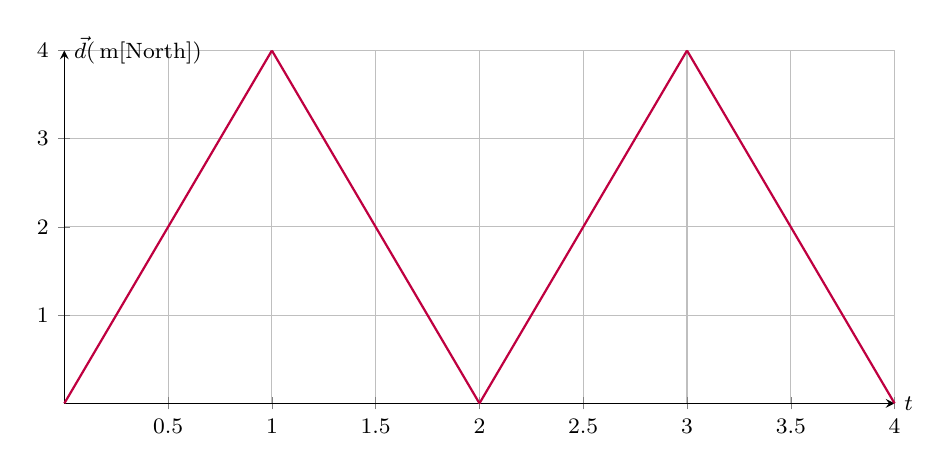
\begin{tikzpicture}
			\begin{axis}[
				my axis style,
				width=\textwidth,
				height=.5\textwidth,
				ylabel=$\vec d (\m \tx{[North]})$,
				grid
			]
			
			\addplot[
				domain=0:1,
				thick,
				purple,
				-
			]
			{4*x};
		
			\addplot[
				domain=1:2,
				thick,
				purple,
				-
			]
			{-4*x + 8};

			\addplot[
				domain=2:3,
				thick,
				purple,
				-
			]
			{4*x - 8};
		
			\addplot[
				domain=3:4,
				thick,
				purple,
				-
			]
			{-4*x + 16};
			
			\fill[
				black
			];
			
			\end{axis}
			\end{tikzpicture}
		\end{center}
	\begin{enumerate}
		\item Which of the following scenarios best describe the motion depicted in the plot,

			\begin{enumerate}[label = (\alph*)]
				\item A ball rolling [North] across a flat road
				\item A sprinter running back and forth at $v_{av} = 4 \m / \s$ on a $4\m$ track.
				\item A man jumping on a trampoline.
			\end{enumerate}
			\textcolor{blue}{\textbf{\underline{Solution: }} b),c)}


		\item Which of the following statements are correct about the plot?
			\begin{enumerate}[label = (\alph*)]
				\item The body experienced uniform motion within the time interval $[1,2]$.
				\item The body experienced uniform motion within the time interval $[0,4]$
				\item Within the time interval $[0,2]$, the average velocity was $\vec v_{av} = +0 \m / \s$.
				\item Within the time interval $[2,3]$, the average velocity was $\vec v_{av} = +4 \m / \ s$.
				\item The average speed within the time interval $[0,4]$ was $v_{av} = 4 \m / \s$.
			\end{enumerate}

			\textcolor{blue}{\textbf{\underline{Solution: }} a),c),d),e)}

		
		\item I label three points on a straight line, $F$, $G$, $H$. Which of the following statements are true?
			\begin{enumerate}[label = (\alph*)]
				\item $\vec d_{FG} = \vec d_{GF} + \vec d_{GH}$
				\item $\vec d_{HF} = (-\vec d_{FG}) + (-\vec d_{HG})$
				\item $\vec d_{FH} = (-\vec d_{GF}) + (-\vec d_{HG})$
				\item $-\vec d_{FG} = \vec d_{GH} + \vec d_{HF}$ \hspace*{4cm} \textcolor{blue}{\textbf{\underline{Solution: }} c),d)}
			\end{enumerate}

	\end{enumerate}
	
\end{qstn}

\begin{qstn}[3]
Covert the following units to $\km / \h$. 
\begin{enumerate}[label = (\alph*)]
	\item $44200 \m / \s$
	\begin{soln}
	$$ 44200 \frac{\cancel{\m}}{\cancel{\s}} \left(\frac{1 \km}{1000\cancel{\m}} \right) \left(\frac{3600 \cancel{\s}}{1\h} \right) = 159120 \frac{\km}{\h} = 1.59 \times 10^5 \frac{\km}{\h}$$
	\end{soln}


	\item $5512 \times 10^4 \inch / \Min$ \hspace*{6cm} (\textbf{1 inch = 2.54cm}, \textbf{1 m = 100 cm})
	\begin{soln}
	$$5512 \times 10^4 \frac{\cancel{\inch}}{\cancel{\Min}} \left(\frac{60 \cancel{\Min}}{1 \h} \right) \left(\frac{2.54 \cancel{\cm}}{1 \cancel{\inch}} \right) \left(\frac{1 \cancel{\m}}{100 \cancel{\cm}} \right) \left(\frac{1\km }{1000 \cancel{\m}} \right) = 84002.88 \frac{\km}{\h}$$
	\end{soln}


	\item $336 \frac{\km}{\text{week}}$
	\begin{soln}
	$$66 \frac{\cancel{\km}}{\cancel{\text{week}}} \left(\frac{1 \cancel{\text{week}}}{7 \cancel{\text{week}}} \right) \left(\frac{1 \cancel{\text{day}}}{24 \h} \right) = 2 \frac{\km}{\h} $$
	\end{soln}



\end{enumerate}


\end{qstn}

\begin{qstn}[4]
	Compute the \textbf{displacement} (or \emph{net} displacement) given the position vectors. Assume that the reference point is $(0,0)$ for \emph{all} vectors.
    \begin{enumerate}[label=(\alph*)]
        \item $\vec d_1 = 514 \tx{\m}[\tx{West}]$, $\vec d_2 = 332 \tx{\m}[\tx{West}]$
		\begin{soln}
		Lets take [East] to be the positive  direction of motion,
			$$\Delta \vec d = \vec d_f - \vec d_i = -332\m - (-514 \m) = +182 \m = 182\tx{m [East]}$$
		\end{soln}


        \item $\vec d_1 = 51 \tx{\m}[\tx{S}]$, $\vec d_2 = 33 \tx{\m}[\tx{S}]$, $\vec d_3 = 27 \tx{\m}[\tx{N}]$, $\vec d_4 = 93 \tx{\m}[\tx{N}]$,$\vec d_5 = 298 \tx{\m}[\tx{S}]$, $\vec d_6 = 432 \tx{\m}[\tx{N}]$


		\begin{soln}
		Lets take [North] to be the positive  direction of motion,
			$$\Delta \vec d = \vec d_f - \vec d_i = +432 \m - (-51\m) = +483\m = 483\tx{m [N]}$$

		\end{soln}



        \item $\vec d_1 = 4\tx{\m}[\tx{East}]$, $\vec d_2 = 4\tx{\m}[\tx{West}]$, $\vec d_3 = 4\tx{\m}[\tx{North}]$, $\vec d_4 = 4\tx{\m}[\tx{East}]$

		\begin{soln}
			Lets take [North] and [East] to be positive direction of motion,
			$$\Delta \vec d =\vec v_f - \vec v_i = +4 - (+4) = +0 = 0\tx{m [East]}$$


		\end{soln}



    \end{enumerate}
\end{qstn}




\begin{qstn}[5]
	Determine the sum/difference of the following vectors \textbf{\emph{geometrically}}. Use the $x-$dimensional coordinate system.
	\begin{enumerate}[label=(\alph*)]
		\item $\vec A = +2$, $\vec B = -8$ $$\vec A + \vec B$$
		\vspace*{3cm}
		\item $\vec A = +4$, $\vec B = -3$, $\vec C = +10$, $\vec D = -12$, $\vec E = -13$, $\vec F = +20$   $$(\vec A + \vec B) - (\vec C - \vec D) + (\vec E - \vec F)$$

	\end{enumerate}
\end{qstn}




\begin{qstn}[6]
	Suppose a train took the following route the other day to the following cities; Oshawa, Pickering, Markham, London (Starting at Oshawa). Given below are all of his position vectors along the trip (All relative to \textbf{Toronto}). Compute his average velocity as well as his average speed if the trip took $4 \h$.
	\begin{itemize}
	\item $\vec d_{OSH} = 224\km$[East]
	\item $\vec d_{PKR} = 154\km$[East]
	\item $\vec d_{MRK} = 72\km$[West]
	\item $\vec d_{LND} = 556\km$[East]
	\end{itemize}

	\begin{soln}
		Let us take [East] as the positive direction of motion. We start by computing the average velocity, this strictly relies on the initial and final position vectors relative to Toronto. The initial position vector relative to Toronto is $\vec d_{OSH} = +224\km$. The final position vector is $\vec d_{LND} = +556$, since it is of course our final location and the vector is already given relative to Toronto. Hence,
		$$\vec v_{av} = \frac{\Delta \vec d}{\Delta t} = \frac{+556 \km - (+224\km)}{4\h} = +83 \km / \h = 82 \km / \h \tx{[East]}$$
		To compute the average speed we must compute all displacements. We analyze the number of displacements the train took throughout the journey. We have the following route $(OSH \rightarrow PKR \rightarrow MRK \rightarrow LND)$, hence you have three displacements which we compute separately.
		\begin{align*}
			\Delta \vec d_1 &= \vec d_{PKR} - \vec d_{OSH} = +154\km - (+224\km) = -70\km\\
			\Delta \vec d_2 &= \vec d_{MRK} - \vec d_{PKR} = -72\km - (+154\km) = -226\km\\
			\Delta \vec d_3 &= \vec d_{LND} - \vec d_{MRK} = +556\km - (-72\km) = +628\km\\
			d &= \sum_i |\overrightarrow{\Delta d_i}|\\
			&= |\overrightarrow{\Delta d_1}| + |\overrightarrow{\Delta d_2}| + |\overrightarrow{\Delta d_3}|\\
			&= |-70 \km| + |-226\km| + |+628\km|\\
			&= 924\km
		\end{align*}
		We can now compute the average speed,
		$$v_{av} = \frac{d}{\Delta t} = \frac{924 \km}{4\h} = 231 \km / \h$$

	\end{soln}

\end{qstn}

\begin{qstn}[8]
	Two tourists, \textcolor{blue}{Tourist A}, \textcolor{red}{Tourist B}, decide to tour a city, below we depict their Position V. Time plots, \emph{however}, we were only able to record information of \textcolor{blue}{Tourist A} after $t = 1$, and information about \textcolor{red}{Tourist B} after $t = 3$. Your task is to determine the equations of motion for both Tourists using the plots given.
	\begin{center}
		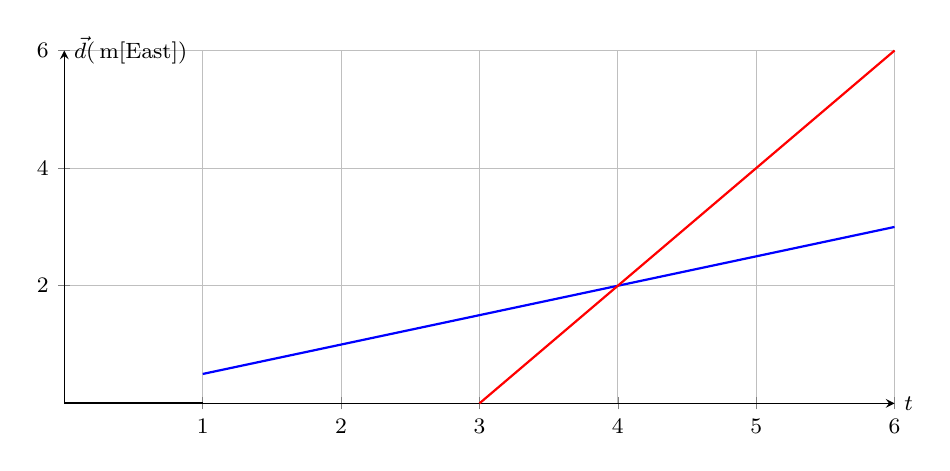
\begin{tikzpicture}
		\begin{axis}[
			my axis style,
			width=\textwidth,
			height=.5\textwidth,
			grid
		]
		
		\addplot[
			domain=1:6,
			thick,
			blue,
			-
		]
		{0.5*x};

		\addplot[
			domain=0:1,
			thick,
			black,
			-
		]
		{0};

		\addplot[
			domain=3:6,
			thick,
			red,
			-
		]
		{2*x - 6};
		
		\fill[
			black
		];
		
		\end{axis}
		\end{tikzpicture}
		\end{center}

		\begin{soln}
			Let the intersection of the two plots be $A(4,2)$. We need to find the linear equations of motion; $\textcolor{blue}{x_A = m_At + b_A}$, $\textcolor{red}{x_B = m_Bt + b_B}$. We first compute the slope the plot and then afterwards determine the y-intercept of each plot,
			\begin{align*}
				\textcolor{blue}{m_A} &= \frac{x_2 - x_1}{t_2 - t_1} \tag{I will use points P1 : (6,3), P2 : (4,2)}\\
				&= \frac{2 - 3}{4 - 6}\\
				&= \frac{1}{2}\\
				\textcolor{red}{m_B} &= \frac{x_2 - x_1}{t_2 - t_1} \tag{I will use points P1 : (6,6), P2 : (4,2)}\\
				&= \frac{2 - 6}{4 - 6}\\
				&= 2
			\end{align*}
			We now have the slope of each plot, we now simply determine the $b$ value for each plot by using a point that exists on their plots. You are free to choose any point, I will choose point $A(4,2)$,
			\begin{align*}
				x_A &= m_At + b_A\\
				x_A &= \frac{1}{2}t + b_A\\
				2 &= \frac{1}{2}\left(4\right) + b_A \tag{Inserting point (4,2)}\\
				b_A &= 0\\
				x_B &= m_Bt + b_B\\
				x_B &= 2t + b_B\\
				2 &= 2(4) + b_B \tag{Inserting point (4,2)}\\
				b_B &= -6
			\end{align*}
			Hence we can construct the equations of motions; 
			$$\textcolor{blue}{x_A = \frac{1}{2}t} \:\:\:\:\: \textcolor{red}{x_B = 2t - 6}$$
		\end{soln}

\end{qstn}


\begin{qstn}[9]
A bunny takes a tour around his neighborhood starting at his shelter. He travels $600\m$[East] to House $A$, then from House $A$ he travels $754\m$[West] to House $B$, then from House $B$ he travels $550 \m$[West] to House $C$, and then finally from House $C$ he travels $2\km$[East] to House $D$. Compute his average velocity as well as his average speed if the elapsed time was $\Delta t = 2\Min$. (Assume that the shelter is the reference point)


\begin{soln}
	Let us assign the [East] direction as the positive direction of motion, for the average velocity we must first obtain the initial position vector relative to the shelter, this happens to simply be $\vec d_I = +0\m$. Next we must obtain the final position vector, the final location the bunny ends up is House $D$, hence we need the position vector $\vec d_{DS}$, where the subscript $S$ represents the shelter. For this we use relative vector math operations, observe that we have the following vectors $\vec d_{AS}, \vec d_{BA}, \vec d_{CB}, \vec d_{DC}$, hence we can apply the relative vector proposition over multiple steps to get to desired result. 
	\begin{align*}
		\vec d_{DB} &= \vec d_{DC} + \vec d_{CB}\\
		&= +2000\m + (-550\m) \\
		&= +1450\m\\
		\vec d_{DA} &= \vec d_{DB} + \vec d_{BA}\\
		&= +1450\m + (-754\m)\\
		&= +696\m\\
		\vec d_{DS} &= \vec d_{DA} + \vec d_{AS}\\
		&= +696\m + (+600\m)\\
		&= +1296\m
	\end{align*}
	Hence the final position vector is $\vec d_F = \vec d_{DS} = +1296$, this allows use to compute the average velocity,
$$\vec v_{av} = \frac{\Delta \vec d}{\Delta t} = \frac{+1296\m}{120\s} = +10.8 \m / \s = 10.8 \m / \s \tx{[East]}$$
The average speed is much simpiler, the question gives us the amount he displaces as he traverses his journey $(A \rightarrow B \rightarrow C \rightarrow D)$. That is, we precisely have all displacement vectors $\Delta \vec d_1 = \vec d_{AS}, \Delta \vec d_2 = \vec d_{BA}, \Delta \vec d_3 = \vec d_{CB}, \Delta \vec d_4 = \vec d_{DC}$. Therefore we compute the distance traveled using the Corollary, afterwards we compute the average speed,
\begin{align*}
	d &= \sum_i |\overrightarrow{\Delta d_i}|\\
	&= |\overrightarrow{\Delta d_1}| + |\overrightarrow{\Delta d_2}| +|\overrightarrow{\Delta d_3}| + |\overrightarrow{\Delta d_4}|\\
	&= |+600\m| + |-754\m| + |-550| + |+2000\m|\\
	&= 600\m  + 754\m + 550\m + 2000\m\\
	&= 3904\m \\
	v_{av} &= \frac{d}{\Delta t} = \frac{3904\m}{120s} = 32.533 \m / \s
\end{align*}
\end{soln}




\end{qstn}

\begin{qstn}[10]
Suppose that I fire an arrow straight up into the air from a cliff at a position $\vec d_{CG} = 56\m$[North] relative to the ground. Suppose that a wooden box $14\m$ high is lying on the ground, and that the arrow lands directly on top of it. Compute the average velocity as well as the average speed of the arrow if the duration of the flight was $\Delta t = 45\s$. (Hint : The reference point is your choice)


\begin{soln}
	Let $A$ denote the subscript of the arrow. Let us choose [North] as the positive direction of motion, let us assign the reference point as the cliff (C). The initial position vector of the arrow (A) relative to the cliff is $d_I = +0\m$. The final position vector $\vec d_{AC}$ of the arrow relative to the cliff may be computed by implementing the relative vector proposition as well as the proposition which states that $-\vec d_{AB} = \vec d_{BA}$. Note that because the arrow lands on a box that is $14\m$ from the ground, the position vector of the arrow relative to the ground is $\vec d_{AG} = +14\m$,
	$$\vec d_{AC} = \vec d_{AG} + \vec d_{GC} =  \vec d_{AG} + (-\vec d_{CG}) = +14\m + (-56\m) = -42\m$$ 
	Hence we have the final position vector $\vec d_f = \vec d_{AC} = -42\m$. We can now compute the average velocity,
	$$\vec v_{av} = \frac{\Delta d}{\Delta t} = \frac{\vec d_F - \vec d_I}{45} = \frac{-42\m - (+0\m)}{45\s} = -0.933 \m / \s$$
\end{soln}



\end{qstn}

\begin{qstn}[11]
	\textcolor{blue}{Runner $A$} and \textcolor{orange}{Runner $B$} run back and forth across a $50\m$ track initially starting at position $(0,0)$ and facing [East] (Assume that [East] is the positive direction of motion). \textcolor{blue}{Runner $A$} has an average speed \textcolor{blue}{$v_{av} = 15 \m / \s$} and \textcolor{orange}{Runner $B$} has an average speed of \textcolor{orange}{$v_{av} = 20 \m / \s$}. After an elapsed time of $\Delta t = 1\Min$, what was the position vector of \textcolor{blue}{Runner $A$} relative to \textcolor{orange}{Runner $B$} (i.e $\vec d_{\textcolor{blue}{A}\textcolor{orange}{B}}$) 


	\begin{soln}
		Let us first determine the amount of time it will take each runner to reach the end of the track, let this time for Runner $A$ be $\textcolor{blue}{\Delta t_A}$ and the time for Runner $B$ to be $\textcolor{orange}{\Delta t_B}$.
		\begin{align*}
			\textcolor{blue}{\Delta t_A }&= \frac{d}{\textcolor{blue}{v_{av}}} = \frac{10}{3}\s \\
			\textcolor{orange}{\Delta t_B} &= \frac{d}{\textcolor{orange}{v_{av}}}= \frac{5}{2} \s
		\end{align*}
	\textbf{\underline{\large{Key Observations:}}}
	\begin{enumerate}
		\item If it takes $\Delta t$ seconds to reach the end of the track, then any integer multiple of $\Delta t \cdot k$ would mean that you have covered the track $k$ times. This means that after $\Delta t \cdot k$ seconds, the runner is either at the start or end of the track.
		\item Let $\Delta t$ be the time it takes for a runner to reach the end of the track. Then by the end of even multiples times of $\Delta t$ ($2\Delta$, $4\Delta t$, etc) correspond to a Runner facing in the [East] direction and by the end of odd multiple times of $\Delta t$ correspond to a Runner facing in the [West] direction. This is because both runners start facing [East], by the end of $\Delta t$, they will begin facing [West], then after $2\Delta$ they will face east again and so on.
	\end{enumerate}
	Observation 1 tells us that if $\Delta t \cdot k = 60$ has an integer solution for $k$, then that Runner is either at the front of the room or at the back of the room. Observation 2 tells us that if $k$ is even then that Runner is facing [East], else he is facing [West]. Lets compute these results,
	\begin{align*}
		\textcolor{blue}{\Delta t_A}\cdot k &= 60\\
		\frac{10}{3}\cdot k &= 60\\
		k &= 18\\
		\textcolor{orange}{\Delta t_B} \cdot k &= 60\\
		\frac{5}{2}\cdot k &= 60\\
		k &= 24
	\end{align*}
	Hence we have found solutions for $k$ for both Runner $A$ and Runner $B$, also both $k$ values are even implying by the end of $60$ seconds, both runners have returned to the start of the track and are at the same location. Hence $\vec d_{\textcolor{blue}{A}\textcolor{orange}{B}} = +0\m$.  

\end{soln}

\end{qstn}

\end{document}



















